\vspace{1cm}

\itshape
En este capítulo se introduce al lector a la teoría en la cual se basa este trabajo de tesis. En la
Sección \ref{sec:terminologia} (página \pageref{sec:terminologia}) se explica brevemente la
terminología que se utiliza a lo largo de este trabajo. Es importante leer esta sección ya que
algunos términos pueden considerarse sinónimos en el habla común, pero en esta tesis, tienen
significados bien diferenciados.

En la Sección \ref{sec:fiabilidad_software} (página \pageref{sec:fiabilidad_software}) explica
qué es la fiabilidad aplicada en sistemas (de software) y cómo se puede clasificar la fiabilidad. En
Sección \ref{sec:impedimentos} (página \pageref{sec:impedimentos}) se detalla el concepto de los
impedimentos de la fiabiliad, cuáles son los orígenes de las fallas, los modos comúnes de fallas
y las fallas en el software.

En la Sección \ref{sec:medios_falla} (página \pageref{sec:medios_falla}) se explican los medios de
la fiabilidad, es decir, los medios para lograr la fiabilidad de sistemas. Aquí se ven los conceptos
de confiabilidad, disponibilidad y seguridad.

La tolerancia a fallas, el núcleo de este trabajo, se explica en la Sección \ref{chap:FaultTolerance}
(página \pageref{chap:FaultTolerance}). En esta sección se detalla el signficado de la tolerancia
fallas, importante para entender este trabajo de tesis.

En la Sección \ref{sec:redundancias_sw} (página \pageref{sec:redundancias_sw}) se explican diferentes
técnicas de redundancias en el software, las cuales son importantes durante el desarrollo
de sistemas críticos.

Las técnicas de evaluación de fiabilidad (Sección \ref{sec:tecnicas_evaluacion_fiabilidad}
\pageref{sec:tecnicas_evaluacion_fiabilidad}) junto con las medidas de fiabilidad
(Sección \ref{sec:medidas_fiabilidad} \pageref{sec:medidas_fiabilidad}) exponen los fundamentos
matemáticos en los cuales se basan los cálculos de tolerancia de fallas. Los métodos de cálculos
de fiabilidad se presentan en la Sección \ref{sec:metodos_calculo_confiabilidad} (página
\pageref{sec:metodos_calculo_confiabilidad})

En la Sección \ref{sec:modelos_fallas} (página \pageref{sec:modelos_fallas}) se explican con más
detalle conceptos importantes tales como, la función de confiabilidad, tasa de falla, tiempo medio
hasta la falla, vida residual media.

En la Sección \ref{sec:protocolos_comunicacion} (página \pageref{sec:protocolos_comunicacion})
se brinda un resúmen teórico de diferentes protocolos de comunicación existentes en la actualidad.

En la Sección \ref{seccion:ProtocoloCAN} (página \pageref{seccion:ProtocoloCAN}) se detalla el
protocolo CAN que es utilizado como principal protocolo de comunicación. La arquitectura propuesta
en este trabajo de tesis utiliza un protocolo de comunicación basado en CAN. En esta sección se describe capa física (página \pageref{subsec:capafisca}), capa de enlace (página \pageref{subsec:capa_enlace}), formato del mensaje (página \pageref{subsec:formato_mensaje}) y se comenta sobre un protocolo basado en CAN que es utilizado en aplicaciones de aeronáutica llamado CANAerospace (página \pageref{subsec:CANaerospace})

\upshape

\noindent\rule{\textwidth}{2pt}
%\begin{center}
%\line(1,0){\textwidth}
%\end{center}
\vspace{1cm}

% section that talk about terminology
% esta seccion habla sobre los términos importantes a utilizar a lo largo de la tesis
\section{Terminología}\label{sec:terminologia}
Existe una importante diferencia entre los significados de las palabras falla, error y
avería\footnote{En inglés: fault, error y failure.}, que es importante destacar antes de comenzar
con el desarrollo de este trabajo.

Un \textbf{avería} de sistema ocurre cuando el servicio prestado por el sistema ya no coincide con
las especificaciones del mismo \citep{Hanmer07}. Esto quiere decir que existe un problema que tiene
una consecuencia negativa en el sistema completo, logrando que este ya no logre cumplir con sus
especificaciones. Cuando el sistema no se comporta de la manera que es especificada, este ha
fracasado. Esto significa que lo que se espera de un sistema se encuentra descripto, comúnmente en
especificaciones o requerimientos \citep{Pullum01}.

Para la \cite{IEEE610.12} avería es ``la inhabilitación de una sistema o componente a llevar a
cabo las funciones requeridas en los requerimientos específicos de perfomance del mismo''.

\cite{Hanmer07} ejemplifica averías de sistemas cuando: el sistema se bloquea y se detiene cuando no
debería hacerlo, el sistema calcula un resultado incorrecto, el sistema no está disponible, el
sistema es incapaz de responder a la interacción con el usuario. Cuando el sistema no hace lo que
debe hacer, el sistema ha fracasado. Las averías son detectados por los usuarios mientras usan el
sistema.

Las averías son causados por los errores. Un \textbf{error} es una parte del estado del sistema
que es susceptible de provocar un avería en el sistema, un error que afecta al servicio es una
indicación de que un avería se ha producido \citep{Hanmer07}. Un error se puede propagar, es decir
dar a lugar otros errores \citep{Pullum01}.

\cite{IEEE610.12} define error como ``la diferencia entre un valor computado, observado o medido,
con el valor verdadero, especificado o el teóricamente verdadero''.

Los errores se pueden clasificar en dos tipos: errores de tiempo y valores \citep{Hanmer07}. Los
errores de valores son aquellos que se manifiestan como valores discretos incorrectos o estados del
sistema incorrecto. En cambio, los errores de tiempo pueden incluir aquellos que no cumplen con el total de las tareas.

\cite{Hanmer07} especifica los siguiente casos más comunes de errores:
\begin{itemize}
 \item Timing: existe una falta de sincronización en la comunicación de los procesos.
 \item Bucles infinitos: ejecución de un bucle sin detenerse, esto consume memoria, y la
avería del sistema.
 \item Error de protocolo: errores en el flujo de comunicación ya que no coinciden los
protocolos. Mensajes enviados en formato diferente, en tiempos diferentes, a lugares de sistemas
incorrectos.
 \item Inconsistencia de datos: errores son diferentes en diferentes lugares.
 \item Sobrecarga de sistema: el sistema es incapaz de hacer frente a la sobrecarga de
actividades a la que es expuesta.
\end{itemize}

La causa adjudicada o la hipótesis de un error es una \textbf{falla}, también llamado ``bugs''. Una
\textbf{falla activa} es aquella que produce un error \citep{Pullum01}. Una falla es un defecto que está
presente en el sistema y que puede causar un error \citep{Hanmer07}. Es la desviación actual de lo
correcto \cite{Hanmer07}.

Según \cite{IEEE610.12} una falla es ``un defecto en un dispositivo de hardware o componente; como
por ejemplo un corto circuito o un cable cortado''. También realiza una segunda definición diciendo
que falla es ``un paso incorrecto, proceso, o definición de dato en un programa de computadora''
\cite{IEEE610.12}. Esta última afirmación es la que se usa en el ámbito de este trabajo.

Algunas fallas introducidas en el \ac{SW} se detallan en \cite{Hanmer07}, lo cual señala que
pueden incluir:
\begin{itemize}
 \item Especificaciones incorrecta de requerimientos
 \item Diseño incorrecto
 \item Errores de programación
\end{itemize}

Entonces, como lo indica \cite{Pullum01} con la tolerancia a fallas, lo que se busca es prevenir la
avería mediante la ``tolerancia'' de fallas, las cuales son detectables cuando un error aparece.
Las fallas son el motivo de errores y los errores son motivos de avería \citep{FTDesign}.

También se suele utilizar el término anomalía en las operaciones de vehículos espaciales para
referirse a comportamientos anómalos o no esperados del sistema \citep{SpaceSystemFailures}

En \cite{FTDesign} se describe un ejemplo para diferenciar correctamente estos conceptos. Se considera
el \ac{SW} de una planta nuclear, en la cual existe una computadora que es responsable de controlar
la temperatura, la presión y demás variables de interés para la seguridad del sistema. Se da el
caso de que uno de los sensores detecta que la turbina principal se encuentra girando a una
velocidad menor a la correcta. Esta falla hace que el sistema envíe una señal para aumentar su
velocidad (error). Esto produce un exceso de velocidad en la turbina, lo cual tiene como
consecuencia que la seguridad mecánica apague la turbina. En esta situación el sistema no está
generando energía. Esto se considera un avería, porque el sistema no está entregando el servicio
según lo establecido por los requerimientos. Pero es un avería salvable.

Otro concepto es el de \textbf{mantenibilidad}, este es la capacidad de un sistema, bajo condiciones normales, de ser restaurado a un estado en el cual puede realizar sus funciones requeridas, cuando se realiza el mantenimiento \citep{Rausand04}.

En secciones posteriores se ven los conceptos de confiabilidad, disponibilidad y seguridad (Sección \ref{subsec:confiabilidad}, \ref{subsec:disponibilidad}, \ref{subsec:seguridad}, respectivamente).


% Section that talk about dependability on software
% TODO:La fiabilidad en el software
\section{La fiabilidad en el software}\label{sec:fiabilidad_software}
El objetivo final de la \ac{FT}, es el desarrollo de un sistema fiable \citep{FTDesign}. Teniendo
en cuenta que \ac{SW} que se encuentra dentro de las naves espaciales, como satélites,
lanzadores, y sobre todo vehículos tripulados son críticos, ya que de ellos dependen el éxito o
fracaso de una misión o la vida de seres humanos,y se debe llevar a cabo un sistema fiable.
La fiabilidad de un sistema es la capacidad del mismo de entregar a los usuarios un nivel
deseado de servicio \citep{FTDesign}.

La fiabilidad también se la puede considerar como una propiedad global que permite justificar la
confianza de los servicios de un sistema \citep{FTAvionics}. Por lo tanto, como lo indica
\cite{FTAvionics} la fiabilidad es un término amplio y cualitativo que está relacionado con
atributos no funcionales (o ``-ilities''), que buscan generar un sistema ``ideal'', especialmente
cuando su funcionamiento es crítico.

Como se muestra en la Figura \ref{fig:dependability_relations} la consecuencia de la fiabilidad es
la relación entre la evitación de fallos y la reducción de fallos, así como también la \ac{FT}.

\begin{figure}[h]
 \centering
 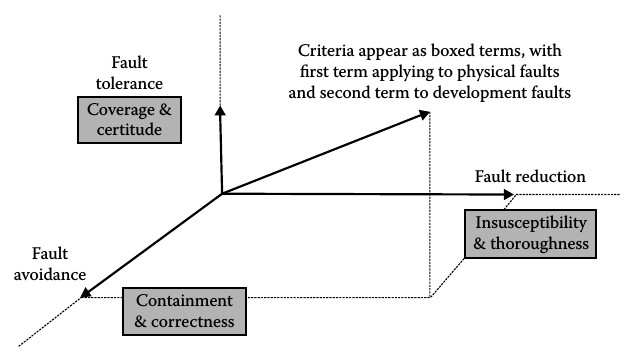
\includegraphics[scale=0.5]{images/Marco_teorico/dependability_relations}
  \caption{Fiabilidad \protect\citep{FTAvionics}}
\label{fig:dependability_relations}
\end{figure}

Según \cite{Pullum01} la fiabilidad puede ser clasificada en:
\begin{itemize}
 \item Impedimentos: son aquellas cosas que se interponen en el camino de la fiabilidad. Son las
fallas, errores y fracasos.
 \item Medios: los medios para lograr la fiabilidad, según el autor, se pueden dividir en dos
grupos:
  \begin{enumerate}
    \item Aquellos que son utilizados durante la construcción del \ac{SW} (\ac{FA}\footnote{En
    inglés, Fault Avoidance} y \ac{FT}).
    \item Aquellos que contribuyen con la validación del \ac{SW} una vez desarrollado
    (\ac{FR}\footnote{En inglés, Fault Removal} y \ac{FF}\footnote{En inglés, Fault Forecasting}).
  \end{enumerate}

 \item Atributos: describen las propiedades de la fiabilidad y proporcionan una forma de evaluar el
logro de esas propiedades.
\end{itemize}

% TODO: deteriodo de la confiabilidad
\section{Impedimentos de la confiabilidad}\label{sec:impedimentos}
El impedimiento de la confiabilidad o deterioro de la confiabilidad es definido en términos de
fallas, errores, y fracaso \citep{FTDesign}. Los mismos fueron desarrollados en la sección
\ref{sec:terminologia}. Lo que tienen en común estos tres conceptos, es que avisan, o dan alerta
cuando algo está mal \citep{FTDesign}. La diferencia radica, en que las fallas son a nivel físico;
los errores se dan a nivel computacional; mientras que los fracaso se dan a nivel de sistema
\cite{FTDesign}.

\subsection{Orígenes de la falla}
Existen diversos orígenes de fallas. Estas pueden provenir desde terceros, en el caso de productos
comprados, pueden deverse a una falta del conocimiento del problema, falta de tiempo, etc.
\cite{FTDesign} clasifica el orígen de las fallas en cuatro grupos: \textit{especificación
incorrecta, implementación incorrecta, defectos de fabricación y factores externos}

Las \textit{especificaciones incorrectas} son aquellas que surgen debidas a una incorrecta
especificación de requerimiento o un mal diseño de una arquitectura o de un algoritmo
\citep{FTDesign}. Estos orígenes de fallas son bastante comúnes en el desarrollo de sistemas. Un
ejemplo típico citado por \cite{FTDesign}, es el caso de requerimientos que ignoran aspectos del
medio ambiente en el que opera el sistema. Una mala redacción de un requerimiento o el olvido de
uno de ellos, puede traer graves problemas, atrasos y pérdida de dinero,  en el diseño y producción
de un sistema espacial.

Las \textit{implementaciones incorrectas}, se refieren a las \textit{fallas de diseño}, surgen
cuando el sistema implementado no cumple con los requerimientos \citep{FTDesign}.

Otro orígen de falla son los \textit{defectos de los componentes} \citep{FTDesign}.Estos pueden
incluir defectos de fabricación, defectos aleatorios dados en los componentes, etc.

Y por último se tienen las fallas que son causadas por \textit{factores externos}, los cuales
provienen del medio ambiente, usuarios u operadores \citep{FTDesign}. Ejemplos de estos factores
externos pueden ser, vibraciones, cargas electroestáticas, temperatura, radición electromagnética,
envío incorrecto de comandos, etc.

% TODO: Modos comúnes de fallas
\subsection{Modos comúnes de fallas}
Un \textit{\ac{CMF}}\footnote{En inglés, common-mode faults} es una falla que ocurre
simultaneamente en dos o más componentes redundantes \citep{FTDesign}.

\cite{Gangloff75} define los \ac{CMF} como múltiples unidades de fracaso debido a una sola causa.

\ac{CMF} son causados por fenómenos que crean dependencias entre unidades redundadas, lo que causa
la falla de estas unidades simultaneamente \citep{FTDesign}.

Según como lo indica \cite{FTDesign} el único enfoque para combatir los \ac{CMF}, es mediante el
diseño en diversidad. Diseño en diversidad es la implementación de más de una variante de la
función en cuestión \citep{FTDesign}. Esto se puede lograr variando los algoritmos que se utilizan,
diferentes equipos de trabajo realicen las mismas partes del sistema, de manera tal de tener
redundancia en código, etc.

%TODO: Fallas en el Software
\subsection{Fallas en el Software}
El \ac{SW} difiere en gran medida con el \ac{HW}. En primer lugar el \ac{SW} no envejece, no se deforma, tampoco se puede quebrar ni ser afectado
por el medio ambiente. El \ac{SW} es determinístico, siempre responde de la misma manera en el mismo ambiente, al menos que falle.

Por otro lado el \ac{SW} se lo puede actualizar varias veces a lo largo del su ciclo de vida.

En tercer lugar, arreglar bugs de \ac{SW} \textbf{no significa que el mismo sea más confiable}, al contrario pueden ocurrir nuevos errores \citep{FTDesign}.

Por último el \ac{SW} es mucho más complejo y menos regular que el \ac{HW}. Tests tradicionales y métodos de debug pueden ser inadecuados para los sistemas de \ac{SW}

% TODO: medios de fiabilidad
\section{Medios de fiabilidad}\label{sec:medios_falla}
Los medios de confiabilidad son métodos y técnicas que permiten el desarrollo de un sistema
confiable \citep{FTDesign}. Los medios se pueden dividir en dos grandes grupos \citep{Pullum01}:
\begin{enumerate}
 \item Aquellos que son empleados durante el proceso de construcción del \ac{SW} \citep{Pullum01},
 \item y a quellos que ayudan en la validación del \ac{SW} después que fue desarrollado
\citep{Pullum01}.
\end{enumerate}

Dentro del primer grupo se tiene:
\begin{itemize}
 \item \acl{FA}
 \item \acl{FT}
\end{itemize}

Por otro lado, en el segundo grupo se puede mencionar los siguientes:
\begin{itemize}
 \item \acl{FR}
 \item \acl{FF}
\end{itemize}

\subsection{\acl{FA}}
\ac{FA} son técnicas de mejoramiento de la fiabilidad utilizadas durante el desarrollo de \ac{SW}
para reducir el número de fallas introducidas durante la etapa mencionada \citep{Pullum01}. Estas
técnicas pueden estar presentes en las especificaciones y requerimientos del sistema, métodos de
diseño de \ac{SW} \citep{Pullum01}.

\cite{FTDesign} la denomina \textit{prevensión de fallas}\footnote{En inglés, Fault prevention}, y
coincide con el autor anterior, definiendo \ac{FA} como técnicas de control de calidad durante la
especificación y fabricación de los procesos de diseño.

% In page 22 of Pullum01 there're more definitions that may be important inside Failure avoidance

\subsection{\acl{FT}}
En la sección~\ref{chap:FaultTolerance} (página~\pageref{chap:FaultTolerance}) se discute con
mayor detalle la \ac{FT}.

\subsection{\acl{FR}}
La \ac{FR} hace referencia a las técnicas utilizadas para mejorar la fiabilidad empleadas durante
la validación y verificación del \ac{SW} \citep{Pullum01}. Estas técnicas mejoran la fiabilidad del
\ac{SW} mediante la detección de fallas, usando métodos de verificación y la validación, y
eliminando las fallas que se van detectando \citep{Pullum01}.

Por otro lado \cite{FTDesign} indica que el \ac{FR} se lleva a cabo durante fases de desarollo de
\ac{SW} tanto como durante el ciclo de vida de un sistema. Durante la fase de desarrollo, \ac{FR}
consiste en tres pasos: \textit{verificación, diagnóstico y correción} \citep{FTDesign}. \ac{FR}
durante la vida operacional de un sistema, consiste en el mantenimiento preventivo y correctivo del
mismo \citep{FTDesign}.

\subsection{\acl{FF}}
La \ac{FF} se realiza mediante la realización de una evaluación del comportamiento del sistema con
respecto a la ocurrencia o la activación de una falla \citep{FTDesign}. Esta evaluación puede ser:
\begin{itemize}
 \item Cualitativa: que tiene como objetivo clasificar los modos de fallas o combinaciones de
eventos que llevan al sistema al fracaso \citep{FTDesign}.
 \item Cuantitativa: que tiene como objetivo evaluar en término de probabilidad, el grado en el
cual los atributos de fiabilidad son satisfechos \citep{FTDesign}.
\end{itemize}

\ac{FF} incluye técnicas para aumentar la fiabilidad del sistema que son usados durante la
validación del \ac{SW}, con el objetivo de estimar la presencia de fallas y la ocurrencia o
consecuencia de fracasos \citep{Pullum01}

% TODO: atributos de la fiabilidad
\section{Atributos de la fiabilidad}\label{sec:atributos_de_la_fiabilidad}
El objetivo final de la \ac{FT} es desarrollar un sistema que sea fiable. Fiabilidad tiene muchas
defini|ciones, pero comúnmente es expresado como la probabilidad de \textbf{no fallar}
\citep{FTAvionics}. ``La fiabilidad es la probabilidad de que un sistema continúe funcionando
correctamente durante un intervalo de tiempo particular'' \citep{SoftwareFaultToleranceATutorial}.

La fiabilidad de un sistema \ac{SW} puede ser descrita por una serie de atributos, los cuales son
mencionados a continuación.

\subsection{Confiabilidad}\label{subsec:confiabilidad}
La confiabilidad es la probabilidad de que un sistema continua operando correctamente durante un
intervalo de tiempo dado \citep{SoftwareFaultToleranceATutorial}.

\cite{FTDesign} coincide que la confiabilidad \textit{R(t)}\footnote{En inlgés, Reliability} de un
sistema es la probabilidad de que el sistema opere sin fracasos en el intervalo de tiempo
\textit{[0,t]}.

La confiabilidad es una medida de la entrega correcta del servicio que brinda un sistema
\citep{FTDesign}.

En sistemas críticos como el \ac{SW} de vehículo espacial, es sumamente necesario que tenga una
alta tasa de confiabilidad, ya que por ejemplo, perder el contacto con la nave, podría representar
la pérdida de la misión, o una gran cantidad de datos. Otro ejemplo que se puede mencionar es de un
satélite geoestacionario de comunicación, la pérdida de este servicio debe ser baja, casi nula
(idealmente).

Coincidiendo, \cite{pressman01} define la confiabilidad como la ``probabilidad de tener operaciones
libre de fallas de un programa de computadora, en un ambiente específico para un tiempo
específico''. El mismo autor también indica que la confiabilidad es la \ac{MTBF}\footnote{Del
inglés, mean-time-between-failure}. Donde:

$$MTBF = MTTF + MTTR$$

El \ac{MTTF} es el promedio de tiempo desde que empieza la operación del sistema hasta el tiempo que
se produce la primera falla. El \ac{MTTR} es el promedio de tiempo que se requiere para recuperarse,
después de un fracaso, al correcto funcionamiento \citep{Hanmer07}. \ac{MTBF}  es similar a
\ac{MTTF}, lo único que los diferencia es que \ac{MTBF} es la suma de \ac{MTTF} y \ac{MTTR}. Según
\cite{Hanmer07}, \ac{MTBF} es utilizado para aquellos sistemas que son reparables. Para el caso
contrario se utiliza \ac{MTTF}.

La \cite{IEEE610.12} define confiabilidad como ``La capacidad del sistema o componente de realizar
sus funciones requeridas bajo las condiciones establecidas durante un período de tiempo
especificado''.

\subsection{Disponibilidad}\label{subsec:disponibilidad}
Es la probabilidad de que el sistema esté operando correctamente en un determinado instante de
tiempo \citep{SoftwareFaultToleranceATutorial}. La disponibilidad \textit{A(t)} de un sistema en el
instante de tiempo \textit{t} es la probabilidad que el sistema esté funcionando correctamente en
el instante \textit{t} \citep{FTDesign}.

\cite{FTDesign} realiza un definción matemática de \textit{A(t)}, llamandola también como
\textit{punto de disponibilidad} o \textit{disponibilidad instantanea}. Y la define como:

$$A(T) = \frac{1}{T} \int_0^T \! A(t) \, \mathrm{d}x $$

Para \cite{Hanmer07} la disponibilidad del sistema es el porcentaje de tiempo en el que es capaz de
llevar a cabo una función determinada.

Para el caso de los sistemas que no pueden ser reperados el punto de disponibilidad es igual a la
confiabilidad del sistema \citep{FTDesign}.

Los estados de disponibilidad pueden ser representados en términos de fuera de servicio por año. En
la Tabla \ref{table:avalVSdowntime} que expone \cite{FTDesign} se puede observar esta relación.

\begin{table}[h]
  \centering
  \begin{tabular}{l|l}
    \hline
    Disponibilidad & Fuera de servicio \\ \hline
    90\%           & 36.5 días/año     \\
    99\%           & 3.65 días/año     \\
    99.9\%         & 8.76 horas/año    \\
    99.99\%        & 52 minutos/año    \\
    99.999\%       & 5 minutos/año     \\
    99.9999\%      & 31 segundos/año   \\ \hline
  \end{tabular}
  \caption{Disponibilidad en relación con su baja de servicio por año. Tabla
modificada de \protect\cite{FTDesign}}
  \label{table:avalVSdowntime}
\end{table}

La \cite{IEEE610.12} define la disponibilidad como ``El grado en el cual un sistema o
componente se encuentra operativo y accesible cuando se requiere su uso. También es expresado en
términos de probabilidad''

En satélites de órbita baja (LEO\footnote{Del inglés, Low Earth Orbit}), es necesario que el
satélite se encuentre disponible al momento de su pasada por las estaciones terrenas, con el fin de 
descargar los datos que se fueron almacenando. Del mismo modo, el satélite debe estar disponible
para llevar a cabo las funciones necesarias, y con esto cumplir con su misión (como por ejemplo la
registración de imágenes en una determinada zona terrestre).

Diferente es el caso para los satélites geoestacionarios, ya que estos deberían estar disponible la
mayor parte del tiempo, ya que en la mayoría de los casos son de comunicación.

\subsection{Seguridad}\label{subsec:seguridad}
La seguridad se considera como una extensión de la confiabilidad \citep{FTDesign}. Seguridad
\textit{S(t)} es definida como la probabilidad que el sistema sea capaz de realizar sus funciones
correctamente o discontinuar sus funciones en una manera a prueba de fallas \citep{FTDesign}.

Según \cite{SoftwareFaultToleranceATutorial} la seguridad es la probabilidad de que el sistema
llevará a cabo sus tareas de una manera no peligrosa. Un peligro se lo puede definir como ``un
estado o condición de un sistema, que juntos con otras condiciones ambientales del sistema,
conducirá inevitablemente a un accidente'' \citep{SoftwareFaultToleranceATutorial}.

La seguridad es requerida para aquellas aplicaciones de seguridad crítica donde un fracaso puede
resultar en lesiones humanas, pérdidas de vida o desastres ambientales \citep{FTDesign}.

En el caso de los satélites, es importante asegurar altos niveles de seguridad, ya que
el fracaso de una misión representa grandes pérdidas de dinero. 


% Section that talk about fault tolerance
%\chapter{Software tolerante a fallas}
\section{Tolerancia a falla}\label{chap:FaultTolerance}
En sistemas críticos, como el de una planta nuclear, sistemas médicos, el sistema de vuelo 
de un avión, o el de un satélite, tanto \ac{SW} (como el hardware) no deben fallar, ya que esto daría 
como resultado la pérdida de vidas humanas, como así también perdidas de dinero.
Para el caso particular, del vehículo espacial 
(satélite, transbordador, lanzador), la falla del \ac{SW} podría tener como consecuencia el
fracaso de una misión, y/o una gran cantidad de dinero, y hasta vidas humanas en algunos caso (como pueden ser en vuelos 
tripulados). La principal diferencia entre el \ac{SW} de una misión satelital, con la de un avión 
o una planta nuclear, o un sistéma médico, es que ante alguna falla o error, se torna complicado 
llegar hasta el satélite para realizar una actualización o cargar un parche de \ac{SW}.

La \cite{IEEE610.12} define como \ac{SW} crítico a ``aquel cuyo fracaso puede tener un impacto en 
la seguridad, o puede causar grandes pérdidas financieras o sociales''. El \ac{SW} de estos 
sistemas críticos deben tener la capacidad de seguir funcionando, aún en la presencia de fallas, o 
errores. Imaginese el caso, de un avión comercial, con pasajeros a bordo, y de repente ocurre un 
problema debido al mal diseño del \ac{SW} (por ejemplo un overflow de memoria). En esta situación 
es impensable que el \ac{SW} se congele y que el piloto reinicie el sistema, esperar que se 
reestablezca al estado en el cual se encontraba antes del problema, para seguir funcionando. Lo 
mismo ocurre con el \ac{SW} de naves espaciales, hay situaciones en la que no se puede esperar y es 
preferible que el sistema siga funcionando aún en la presencia de fallas.

Tal como lo indica \cite{pressman01} las fallas de \ac{SW} implican problemas cualitativos que son 
descubiertos después de que el \ac{SW} es llevado a los usuarios y probados por ellos. Una 
gran cantidad de estudios indican que en las actividades de diseño se introducen entre un 50 y 65 
porciento de errores del total de errores que se dan durante el proceso del \ac{SW} 
\citep{pressman01}. Esto no debe ocurrir en el ámbito espacial, ya que una vez que el sistema es 
utilizado, es muy difícil corregir los errores que surgen 

Cabe aclarar que el \ac{SW} al no ser un componente físico, no puede ser tratado de la misma 
manera que un componenete hardware. Como ejemplifica \cite{SoftwareFaultToleranceATutorial}, las 
fallas que surgen a nivel de bit, como por ejemplo en un disco duro, son fallas del dispositivo de 
almacenamiento y pueden ser mitigadas con la aplicación de técnicas de redundancias. Esto no es así 
para el \ac{SW}. Por lo tanto evitar los errores a nivel de \ac{SW} no es tan trivial como 
en el hardware.

A nivel de \ac{SW} las fallas son llamadas ``bugs'' (tal como se indica en la
sección~\ref{sec:terminologia} en la página~\pageref{sec:terminologia}), y existe 
un solo tipo de fallas que es introducido durante el desarrollo del \ac{SW} 
\citep{SoftwareFaultToleranceATutorial}. Las fallas en el \ac{SW} son el principal motivo de que 
todo un sistema fracase. 

La \ac{FT}, puede ser utilizada como una capa más de protección 
\citep{SoftwareFaultToleranceATutorial}. Esta aplicada al \ac{SW} se refiere al uso de técnicas que 
permiten seguir brindando el servicio en un nivel aceptable de perfomance y seguridad después que 
una falla de diseño ocurra. 

Debe hacerse una diferencia entre \ac{FT} y calidad. \cite{Hanmer07} lo define de la 
siguiente manera: ``\ac{FT} es la capacidad del sistema a ejecutarse apropiadamente a 
pesar de la presencia de fallas. \ac{FT} ocurre en tiempo de ejecución''. Cuando se 
habla que un sistema es tolerante a fallas, significa que fue diseñado de tal manera, que 
puede seguir funcionando correctamente aún en la presencia de errores de sistemas \citep{Hanmer07}. 

En cambio calidad, tal como lo define \cite{Hanmer07}, ``se refiere a cuán libre de fallas está el 
sistema. Técnicas de calidad que indican cómo el \ac{SW} es creado. Si el sistema fue testeado.'' 

Un sistema de alta calidad tendrá menor número de fallas, que esto representa menor número de 
fallas en tiempo de ejecución. La reducción del número de fallas no implica que los resultados de 
los defectos son menos severos \citep{Hanmer07}. El sistema debe tomar medidas para reducir el 
impacto de los errores y fallas, y es allí donde surge la \ac{FT}.	

Un sistema tolerante a fallas provee una continua y segura operación, aún durante la presencia 
de fallas. Un sistema tolerante a fallas, es un elemento crítico para una arquitectura de vuelo, lo 
cual incluye hardware, \ac{SW}, timing, sensores y sus interfaces, actuadores, elementos y datos 
de comunicación con los diferenes elementos \citep{FTAvionics}. 

Este tipo de sistemas debería detectar los errores causados por fallas, evaluar los daños 
producidos por la falla, aislar a la misma y por último recuperarse, en ese caso se habla de 
aquitectura o sistemas \acs{FDIR}\footnote{FDIR, del inglés: Failure detect, isolate and recover}.

\ac{FT} es la capacidad de un sistema a continuar funcionando a pesar de la ocurrencia 
de fallas \citep{FTDesign}. Un sistema tolerante a fallas debe ser capaz de manejar fallas tanto de 
hardware como de \ac{SW}. La \ac{FT} es necesaria debido a que es imposible construir 
un sistema perfecto.

El objetivo de la \ac{FT} es el desarrollo de sistemas que tengan la capacidad de
funcionar correctamente en 
presencia de fallas \citep{FTDesign}. La \ac{FT} es alcanzada mediante la utilización de redundancias \citep{FTDesign}. \textit{Redundancia} es la provisión de capacidades 
funcionales que sería innecesario para entornos libres de fallas \citep{FTDesign}. Esto significa 
tener hardware adicionales, check bits en una cadena de datos, o algunas l\'ineas de c\'odigo que 
verifique el resultado correcto del \ac{SW}. La redundancia permite enmascarar una falla, o 
detectarla, para luego localizarla, contenerla y recuperarse de esta \citep{FTDesign}. Las 
técnicas de tolerancia de fallas se emplean durante la adquisición, o desarrollo del \ac{SW}. 
Permite al \ac{SW} tolerar fallas después que este haya sido desarrollado \citep{Pullum01}. Cuando 
una falla se da, las técnicas de \ac{FT} proveen mecanismos al sistema de \ac{SW} para prevenir el 
fracaso del sistema \citep{Pullum01}.

%\section{Clasificación de un sistema de control tolerante a fallas}

\section{Redundancia en el software}\label{sec:redundancias_sw}
A pesar de lo comentado anteriormente, sobre la importancia del \ac{SW}, todavía existe una 
creencia, de que el \ac{SW} aparece por arte de magia, y que los programadores no son nunca, lo 
suficientemente capaces, de hacer un \ac{SW} libre de errores. Salvo aquellas empresas u 
organizaciones que tienen un proceso maduro de desarrollo de \ac{SW}, el resto suele encasillarse
en el pensamiento mencionado anteriomente. 

\cite{FTDesign} explica que la \ac{FT} aplicado en el \ac{SW} no está tan entendido, ni maduro, 
como es en el caso de la \ac{FT} aplicada en hardware. Si una falla exisitiera en el \ac{SW}, esta 
se haría ``visible'', solo cuando las condiciones relevantes ocurran \citep{FTDesign}. Y muchas 
veces por tiempo o costo, no se realizan los tests cubriendo todos los posibles ambientes reales, 
lo cual tiene consecuencias desastrosas, tal como se expone en la sección~\ref{chap:motivacion} 
(página~\pageref{chap:motivacion}).

Para sistemas complejos o grandes, donde existe una gran cantidad de estados, implica que solo una 
pequeña porción del \ac{SW} puede ser verifcada correctamente \citep{FTDesign}. Los tests 
tradicionales y métodos de depuración actuales no alcanzan para grandes sistemas \citep{FTDesign}. 
La utilización de métodos formales para describir las característica requeridas por el 
comportamiento del \ac{SW} exigen gran complejidad computacional, y solo son aplicables en 
ciertas situaciones \citep{FTDesign}.

Las técnicas de \ac{FT} se pueden dividir en dos grupos:
\begin{itemize}
 \item técnicas de una sola versión (single version), se utilizan cuando existe una sola versión del \ac{SW} en el 
sistema.
 \item técnicas multi-versión (multi-version), se utilizan cuando se desarrollan varias versiones de una misma 
función. 
\end{itemize}

Estas se explican en las siguientes secciones.

\subsection{Técnicas single version}
Estas técnicas son utilizadas para tolerar parcialmente las fallas del diseño de \ac{SW} 
\citep{Pullum01}. Técnicas single-version de \ac{FT} se basa en el uso de redundancia aplicada a 
una única versión de una pieza de \ac{SW} para detectar y recuperarse de fallas 
\citep{SoftwareFaultToleranceATutorial}. 

Estas técnicas le brindan a los software que cuentan con una sola versión, un número de capacidades funcionales 
que no serían necesarias dentro de un ambiente libre de fallas \citep{FTDesign}. 

\subsubsection{Estructuras de software}
En \cite{SoftwareFaultToleranceATutorial} se mencionan dos técnicas de estructuración del \ac{SW}
que presentan características favorables al momento de mantener \ac{FT} en el \ac{SW}.

La definición de una arquitectura en el software es de suma importancia ya que proveen las bases para 
la implementación de \ac{FT} \citep{SoftwareFaultToleranceATutorial}. Una de las técnicas utilizadas 
en el desarollo del software es la modularización. Esta consiste en descomponer el problema en 
componentes manejables. Esto tiene como resultado que sea más eficiente la aplicación de la \ac{FT} 
en el diseño de un sistema \citep{SoftwareFaultToleranceATutorial}. 

El particionado es otra técnica mencionada en \cite{SoftwareFaultToleranceATutorial}, lo cual 
provee aislación entre módulos independentes del sistema. Esta técnica permite descomponer al 
problema en partes separadas \citep{pressman01}. El particionado puede ser horizontal u 
vertical. En el primero se descompone el problema moviéndose en forma horizontal en la jerarquía, 
mientras que el segundo se parte de lo más general hasta llegar a lo detallado, moviendose 
verticalmente en la jerarquía \citep{pressman01}. 

Sistema de cierre es un principio de \ac{FT}, en el cual ninguna acción es permitible sin una 
autorización expresa \citep{SoftwareFaultToleranceATutorial}. Siguiendo este principio ninguna de 
las funciones que componen al sistema deberían tener más capacidad de la necesaria 
\citep{SoftwareFaultToleranceATutorial}. Las ventajas de desarrollar un sistema bajo este principio, 
es que es sencillo el manejo de errores, y evitar la propagación de fallas si ocurriesen. 

\subsection{Técnicas multi-version}
Las técnicas de multi-version utilizan dos o más versiones diferentes del mismo módulo de \ac{SW} 
(\citep{FTDesign}; \citep{SoftwareFaultToleranceATutorial}), lo cual satisface el requerimiento de 
diversidad. 

El objetivo de utilizar diferentes versiones de \ac{SW} es que es construido de diferentes 
maneras, por lo tanto fallarían de diferente maneras \citep{SoftwareFaultToleranceATutorial}.

\subsection{Técnicas de detección de fallas}
Para los \ac{SW} tolerantes a fallas de una sola versión, se suelen utilizar varios tests de 
``aceptación'' para detectar fallas \citep{FTDesign}. Es necesario que estos \ac{SW} cuenten con 
dos propiedades: auto protección\footnote{En inglés, self-protection} y auto check\footnote{En 
inglés, self-checking} \citep{SoftwareFaultToleranceATutorial}. La auto protección significa que  
los componentes del sistema tienen la capacidad de protegerse así mismo mediante la detección de 
errores \citep{SoftwareFaultToleranceATutorial}. La propiedad de auto check significa que los 
componente son capaces de detectar fallas internas y tomar las acciones necesarias para evitar la 
propagación del error. 

El resultado del sistema depende del resultado de los tests. Si el resultado pasa exitosamente el 
test, este es el correcto, caso contrario significa la presencia de fallas \citep{FTDesign}. Un test 
es más efectivo si se puede calcular de una manera simple \citep{FTDesign}. 

Las técnicas utilizadas son las siguientes:
\begin{itemize}
 \item \textit{Timing checks:} se agrega a los sistemas una restricción de tiempo. Basado en esa 
restricción se puede deducir si el comportamiento del sistema se desvió \citep{FTDesign}. Los más 
utilizado es el \textit{watchdog timer}, este es un contador que se actualiza con un \textit{timer} que 
detecta si un módulo de \ac{SW} se bloqueó o congeló, entonces se reinicia ese módulo o el sistema. 
 \item \textit{Coding checks:} se utiliza en los sistemas donde los datos se codifican usando 
técnicas de redundancia de datos \citep{FTDesign}. 
 \item \textit{Reversal checks:} son aquellos donde se toma los valores de salida, y con ellos se 
busca encontrar cuáles fueron los datos de entrada. Si los datos de entrada reales coinciden con 
los calculados (para una misma salida), este se encuentra libre de fallas \citep{FTDesign}. 
 \item \textit{Reasonableness checks:} usa propiedades semánticas en los datos para detectar 
fallas \citep{FTDesign}. 
 \item \textit{Structural checks:} se basa en el conocimiento de las propiedades de la estructura 
de datos \citep{FTDesign}. 
 \item \textit{Replication checks: } se basa en la comparación de resultados de varios componentes 
\citep{SoftwareFaultToleranceATutorial}. 
\end{itemize}

Se suelen utilizar árboles de fallas, como una técnica auxiliar en el desarrollo de sistemas para 
la detección de fallas \citep{SoftwareFaultToleranceATutorial}. El árbol de falla permite obtener 
un enfoque top-down de las diferentes fallas que se pueden dar. El árbol no cubre todas las fallas 
que puedan darse, pero si ayudan en un alto grado en el desarrollo de \ac{SW} tolerante a fallas 
\citep{SoftwareFaultToleranceATutorial}. 

\subsection{Técnicas de recuperación de fallas}
Una vez que la falla es detectada, el sistema debe proceder a recuperarse de aquella, y volver a 
un estado operacional normal \citep{FTDesign}. Si los mecanismos de deteccíón y contención de 
fallas fueron desarrollados correctamente, esta es contenida dentro de un set de módulos en el 
momento de la detección \citep{FTDesign}. 

\subsubsection{Manejo de excepciones}
En muchos \ac{SW} y lenguajes de programación, los errores se pueden recuperar mediante el manejo de 
excepciones. El manejo de excepciones es la interrupción del funcionamiento normal para responder a 
un funcionamiento anormal del sistema \citep{SoftwareFaultToleranceATutorial}. Los posibles eventos 
que pueden lanzar una excepción son:
\begin{enumerate}
 \item Excepciones de interfaces, son lanzadas por un módulo cuando se da una solicitud inválida de 
algún servicio \citep{FTDesign}.
 \item Excepciones locales, son lanzadas por algún módulo cuando sus propios mecanismos de 
detección de fallas encuentran un problema interno \citep{FTDesign}.
 \item Excepciones de fracaso, son lanzadas cuando un mecanismos de detección encuentra una falla, 
pero es imposible recuperarse de esa falta \citep{FTDesign}.
\end{enumerate}

\subsubsection{Checkpoint y Restart}
Para los software de una sola versión existen pocos mecanismos de recuperación. Checkpoint y restart 
es uno de ellos. También es conocido como \textit{backward error recovery} \citep{FTDesign}. La 
mayoría de las fallas que se dan en los \ac{SW} son debido a fallas que provienen del diseño, tal 
como se mencionó anteriomente. Estas fallas son activadas por entradas al sistema \citep{FTDesign}. 

Este mecanismo cuenta con el módulo principal que se encuentra en ejecución combinado con un bloque 
que realiza tests de aceptación. Si se detecta una falla, en el bloque de testeo, se envía una 
señal de ``reincio'', para que el módulo principal vuelva al estado anterior, es decir, antes de 
producirse el error. Este estado anterior se encuentra almacenado en una memoria checkpoint 
\citep{FTDesign}. En la figura \ref{fig:checkAndRestart}\footnote{Basado en \cite{FTDesign} y 
\cite{SoftwareFaultToleranceATutorial}}, se muestra la representación de este mecanismo.

\begin{comment}
\begin{figure}[h]
  \centering
  \begin{tikzpicture}
  % definicion de estilos
  \tikzstyle{cuadro} = [draw, sep=5,rectangle,minimum height=3em, minimum width=6em, node 
  distance=2cm] 

  \tikzstyle{vacio} = [inner, sep=5,rectangle,minimum height=3em, minimum width=6em, node 
  distance=3cm] 

  \tikzstyle{circulo} = [fill, shape=circle, minimum size=5pt, inner sep=3pt, node distance=4cm ]
  
  % cuadros
  \node[cuadro] (checkMemo){Memoria de Checkpoint};
  \node[cuadro , below of=checkMemo, pin={[->] left:Entrada}] (modulo){Módulo en ejecución};
  \node[circulo, right of=modulo] (circ){};
  \node[cuadro, below of=circ] (detector){Test de aceptación};
  \node[vacio, right of = circ] (salida){Salida};

  \draw[->] (checkMemo.-30)--(modulo.30);
  \draw[->] (modulo.150) -- (checkMemo.-150);
  \draw[->] (modulo)--(circ);
  \draw[->] (circ)--(salida);
  \draw[->] (circ)--(detector);
  \draw[->] (detector)-|(modulo) node[near end, left] {retry};
  \end{tikzpicture}
  \caption{Representación de checkpoint y restart}
  \label{fig:checkAndRestart}
\end{figure}
\end{comment}

\begin{figure}[h]
 \centering
 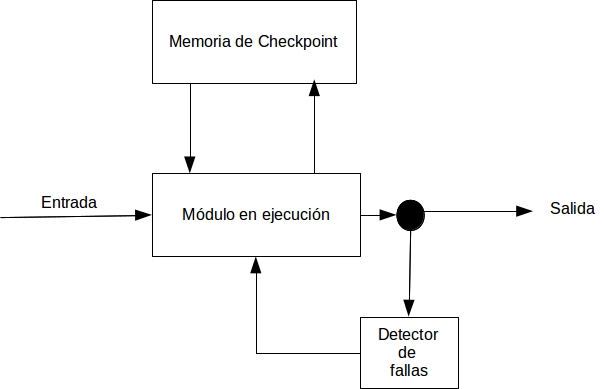
\includegraphics[scale=0.5]{images/Marco_teorico/checkAndRestart.jpg}
 \caption{Representación de checkpoint y restart}
 \label{fig:checkAndRestart}
\end{figure} 


Existe dos tipos de checkpoints, estáticos y dinámicos. Los checkpoints estáticos toman una 
``fotografía'' del estado del sistema antes de comenzar la ejecución del \ac{SW} y lo guarda en la
memoria \citep{FTDesign}. Si se detecta una falla, el sistema regresa a ese estado y 
comienza de nuevo su ejecución \citep{FTDesign}. Los checkpoints estáticos se basan en regresar el 
módulo a un estado predeterminado \citep{SoftwareFaultToleranceATutorial}. Se puede regresar a un 
estado inicial o a un set de estados predeterminados \citep{SoftwareFaultToleranceATutorial}.

Por otro lado se encuentran los checkpoints dinámicos. Estos usan checkpoints creados 
dinámicamente. Estas son imágenes del estado del sistema en varios puntos durante la ejecución 
\citep{SoftwareFaultToleranceATutorial}.

Hay tres formas de crear los checkpoints dinámicamente:
\begin{enumerate}
 \item Equidistantes, en el cual los intervalos que se crean los checkpoints son siempre iguales, 
los intervalos se elijen teniendo en cuenta el rate de falla \citep{FTDesign}. 
 \item Modular, en el cual los checkpoints se crean al principio o al final de la ejecución de un 
módulo. 
 \item Random, los checkpoints se crean aleatoriamente en el tiempo. 
\end{enumerate}

\subsubsection{Procesos pares}
Los procesos a pares utilizan dos versiones idénticas de un proceso de \ac{SW} que corre en 
procesadores separados (\citep{FTDesign}; \citep{SoftwareFaultToleranceATutorial}). El mecanismo de 
recuperación que se utiliza es el de checkpoint y restart \citep{SoftwareFaultToleranceATutorial}.  

Como se puede observar en la figura~\ref{fig:repPares}\footnote{Basada en \cite{FTDesign} y 
\cite{SoftwareFaultToleranceATutorial}} el primer procesador se encuentra activo. Este envía un 
checkpoint al segundo procesador. Si una falla se detecta, el primer procesador se apaga y se cambia 
al segundo procesador. El segundo procesador carga el checkpoint y continua con la operación.Toma el 
rol del primer procesador \citep{SoftwareFaultToleranceATutorial}. Luego el 
primer procesador realiza un auto test para verificar si el problema continua. Si se encuentra que 
este procesador sigue teniendo problema, se continúa trabajando con el segundo procesador 
\citep{FTDesign}.

La principal ventaja que brinda este mecanismo según \cite{FTDesign} es que permite entregar el 
servicio ininterrumpidamente.

\begin{figure}[h]
 \centering
 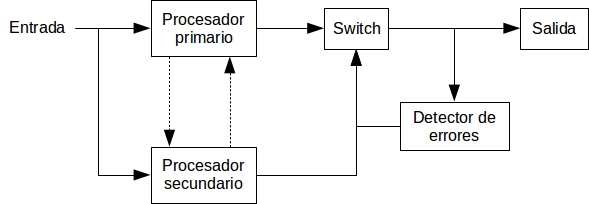
\includegraphics[scale=0.6]{images/Marco_teorico/repPares.jpg}
 \caption{Representación del proceso pares}
 \label{fig:repPares}
\end{figure} 

\begin{comment}

\begin{figure}[h]
 \centering
 \begin{tikzpicture}[node distance=1cm, auto,]
  % definicion de estilos
  %Define style for boxes
   \tikzset{
   cuadro/.style={
           rectangle,
           draw=black,
           text width=6.5em,
           minimum height=2em,
           text centered},
    % Define arrow style
    arrow/.style={
           ->,
           thick,
           shorten <=2pt,
           shorten >=2pt,}	
    }
  \tikzstyle{circulo} = [draw, fill=black, circle, node distance=1cm, minimum size=5pt, inner 
sep=3pt]
    
  % Gráfico
  \node[inner sep=5pt] (entrada) {Entrada};
  \node[cuadro, right=0.5cm of entrada] (prim) {Procesador Primario};
  \node[cuadro, inner sep=5pt,below=0.5cm of prim] (secu) {Procesador Secundario};
  \node[cuadro, inner sep=10pt, right=1cm of prim] (selec) {Switch};
  \node[inner sep=0pt, right=2cm of selec](ghost1){};
  \node[cuadro, below=0.5cm of ghost1](detector) {Detector de error};
  \node[inner sep=0pt, right=0.5cm of ghost1] (salida) {Salida};
  
  \draw[arrow] (entrada)--(prim);
  \draw[arrow] (entrada)|-(secu);
  \draw[arrow, dashed] (prim.-30) -- (secu.30);
  \draw[arrow, dashed] (secu.150) -- (prim.-150);
  \draw[arrow] (prim)--(selec);
  \draw[arrow] (secu)-|(selec.-150);
  \draw[arrow] (detector)-|(selec);
  \draw[arrow] (selec)--(salida);
  \draw[arrow] (ghost1)--(detector);
 \end{tikzpicture}
 \caption{Representación del proceso pares}
 \label{fig:repPares}
\end{figure}

\end{comment}

\subsubsection{Diversidad de datos}
La diversidad es una técnica utilizada para mejorar la eficiencia en los checkpoint y restart, 
usando diferentes entradas por cada reinicio. Esto se basa en que las fallas en el 
\ac{SW} son dependientes de las entradas. Es poco probable que la misma falla se 
de con la misma secuencia de entrada \citep{FTDesign}.

\subsubsection{Bloques de recuperación}

Esta técnica combina las bases de la técnica de checkpoints y restart enfocada con múltiples 
versiones de un componente de \ac{SW} en el sentido de que una versión de \ac{SW} diferente es 
lanzada cada vez que se encuentra una falla. Los 
checkpoints son creados antes de que una versión de \ac{SW} se ejecuta.
La ejecución de las múltiples versiones pueden ser 
secuencial o paralelas dependiendo de la disponibilidad de la capacidad de procesamiento y 
perfomance requerida \citep{SoftwareFaultToleranceATutorial}.

%La representación de esta técnica se puede observar en el figura~[AGREGAR IMAGEN].
Las 
versiones son diferentes implementaciones de un mismo programa. Solo una de estas versiones provee 
la salida del sistema. Si un error es detectado por el test de aceptación, se vuelve hacia atrás, 
se retoma el último checkpoint, y se vuelve a ejecutar el módulo de \ac{SW} pero con una 
versión diferente a la que se ejecutó anteriormente \citep{FTDesign}.  	

Los checks del test de aceptación deben mantenerse simples para mantener la velocidad de la 
ejecución \citep{FTDesign}.

\begin{comment}
\begin{figure}[h]
 \centering
 \begin{tikzpicture}[node distance=1cm, auto,]
  % definicion de estilos
  %Define style for boxes
   \tikzset{
   cuadro/.style={
           rectangle,
           draw=black,
           text width=6.5em,
           minimum height=2em,
           text centered},
    % Define arrow style
    arrow/.style={
           ->,
           thick,
           shorten <=2pt,
           shorten >=2pt,}	
    }
       
  \tikzstyle{circulo} = [draw, fill=black, circle, node distance=1cm, minimum size=5pt, inner 
sep=3pt]
    
  % Gráfico
  \node[inner, sep=5pt] (input1){Entrada 1};
  \node[inner, sep=5pt, below=0.5cm of input1] (input2){Entrada 2};
  \node[inner, sep=5pt, below=0.5cm of input2] (puntos1){...};
  \node[inner, sep=5pt, below=0.5cm of puntos1] (inputn){Entrada n};
  \node[cuadro, right=0.5cm of input1] (version1){Versión 1};
  \node[cuadro, right=0.5cm of input2] (version2){Versión 2};
  \node[inner, sep=5pt, right=2cm of puntos1](puntos2){...};
  \node[cuadro, right=0.5cm of inputn] (versionn){Version n};
  
  \node[cuadro, above=1cm of version1] (check) {Memoria Checkpoint};
  \node[cuadro, right=1cm of version2] (switch) {Swith n a 1};
  \node[inner, sep=0pt, right=1cm of switch](ghost1){};
  \node[cuadro, below=0.5cm of ghost1](test){Test de aceptación};
  
  \node[inner, sep=0pt, right=0.5cm of ghost1](output){Salida};
 
  %Arrows
  \draw[arrow] (input1)--(version1);
  \draw[arrow] (input2)--(version2);
  \draw[arrow] (inputn)--(versionn);
  \draw[arrow] (version1)-|(switch.west);
  \draw[arrow] (version2)--(switch);
  \draw[arrow] (versionn)-|(switch.west);
  \draw[arrow] (ghost1)--(test);
  \draw[arrow] (switch)--(output);
  
  \draw[arrow, dashed] (check.-40) -- (version1.30);
  \draw[arrow, dashed] (version1.150) -- (check.-145);
  
  

 \end{tikzpicture}
 \caption{Configuración de bloques de recuperación}
 \label{fig:repPares}
\end{figure}
\end{comment}

%\subsubsection{Programación N-version}

%\subsubsection{Programación N-Auto Checking}



%Section that talk about dependability evaluation techniques
\section{Técnica de evaluación de fiabilidad}
La evaluación de la fiabilidad es de suma importancia para el desarrollo de sistemas críticos, ya
que permite identificar que aspectos del comportamiento del sistema juega un papel importante
\citep{FTDesign}.

\begin{enumerate}
 \item Modelado de un sistema en la fase de diseño.
 \item Aseguramiento del sistema en la fases finales de desarrollo (testing).
\end{enumerate}
El análisis confiabilidad tiene tres enfoques importantes:
\begin{itemize}
  \item Confiabilidad de \ac{HW}
  \item Confiabilidad de \ac{SW}
  \item Confiabilidad humana
\end{itemize}
En este trabajo de tesis se pondrá énfasis en el estudio en la confiabilidad del \ac{SW} a nivel de sistema.

La evaluación de la fiabilidad tiene dos aspectos. En primer lugar se tiene una \textit{evaluación
cualitativa} que permite identificar, clasificar y medir modos de fallas, o eventos combinacionales
que puedan provocar una falla. El otro aspecto es la \textit{evaluación cuantitativa}, la cual
permite evaluar en términos de probabilidad los atributos de la fiabilidad (Sección \ref{sec:atributos_de_la_fiabilidad}), disponibilidad, seguridad.

El análisis de confiabilidad es de gran importancia ya que provee información que es la base de la toma de desición. Esto es aplicado a diferentes áreas, tales como análisis de riesgos, protección ambiental, calidad, optimización de mantenimientos y operaciones y diseño de ingeniería \citep{Rausand04}.

\section{Medidas comunes de fiabilidad}
Las medidas de fiabilidad más comunes son las siguientes: failure rate, tiempo medio a la falla,
tiempo medio de reparación y tiempo medio entre fallas.

\subsection{Failure rate}
Failure rate $\lambda$ es el número esperardo de fallas por unidad de tiemp \citep{FTDesign}. Es
usual utilizar la dimensión \textit{fallas/horas}.

Generalmente, $\lambda$ se encuentra a nivel de componente. Para conocer el failure rate del
sistema completo, se puede realizar (a groso modo) una sumatoria de los $\lambda$ de los
componentes que integran el sistema. $$\lambda=\sum_{i=1}^{n} \lambda_i$$.

La evolución de $\lambda$ a través del tiempo, no tiene el mismo comportamiento tanto para \ac{HW} como para \ac{SW}
Si se devide el ciclo de vida de un sistema en las siguientes fases: mortalidad prematura (I), vida útil (II), desgaste (II) \citep{FTDesign}
se aprecia, para el caso del \ac{HW}, lo que se denomina \textit{curva de la bañera} la cual puede observarse en la Figura \ref{fig:bathtub_curve}.
En una primera fase, $\lambda$ decrese, ya que a través de los procesos de testing se van descubriendo y resolviendo los errores. Luego se da un periodo de estabilización.
Y al final, el \ac{HW} sufre el paso del tiempo, y se desgasta, aumentando la tasa de fallas.

\begin{figure}[h]
 \centering
 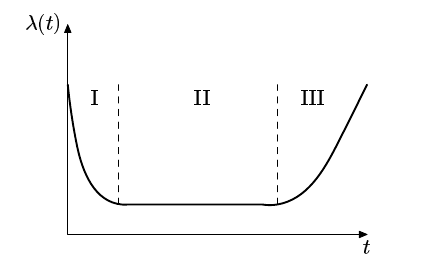
\includegraphics[scale=0.5]{images/Marco_teorico/bathtub_curve.png}
  \caption{Failure rate de HW vs tiempo }
\label{fig:bathtub_curve}
\end{figure}

Para el \ac{SW} es totalmente diferente. En primer lugar cuando se realiza una actualización, se aumenta la complejidad, como así también la probabilidad de fallas,
con ello el failure rate. Otra diferencia sustancia con el \ac{HW} es que el \ac{SW} no se desgasta con el tiempo. En la Figura \ref{fig:Failure_rate_software}
se aprecia $\lamda$ a través de tiempo. Esta curva suele llamarse \texit{curva serrucho}. El failure rate del \ac{SW} decrece en función del tiempo. En estos tipo de sistemas
la tasa de falla depende de varios factores como pueden ser el proceso utilizado en el diseño y codificación, complejidad del \ac{SW}, tamaño del \ac{SW},etc \citep{FTDesign}.

\begin{figure}[h]
 \centering
 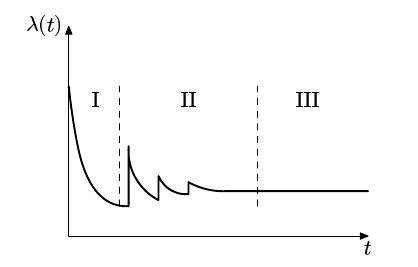
\includegraphics[scale=0.5]{images/Marco_teorico/Failure_rate_software.png}
  \caption{Failure rate SW vs tiempo }
\label{fig:Failure_rate_software}
\end{figure}

A lo largo de la vida de sistema se supone el failure rate $\lambda$ como constante. Por lo tanto la confiabilidad del sistema varía exponencialmente
con respecto al tiempo \citep{FTDesign}: $$R(t) = e^{- \lambda t}$$

Esto se conoce como \textit{ley de la falla exponencial}\citep{FTDesign}. El gráfico de confiabilidad $R(t)$ vs tiempo se muestra en la Figura \ref{fig:failure_rate}.

\begin{figure}[h]
 \centering
 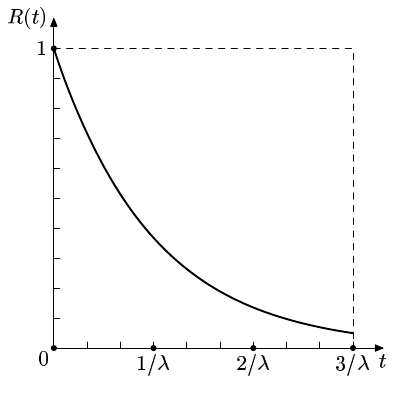
\includegraphics[scale=0.5]{images/Marco_teorico/failure_rate.png.png}
  \caption{Confiabilidad vs tiempo }
\label{fig:failure_rate}
\end{figure}

\subsection{Tiempo medio medio de falla}
\textit{El tiempo medio de falla} (MTTF\footnote{Del inglés, Mean Time To Failure}) de un sistema es el tiempo esperado que transcurra hasta la primera falla que se
detecte en el sistema. En terminos de confiabilidad, MTTF se define de la siguiente manera \citep{FTDesign} \citep{Rausand04} $$\int_0^{\infty} R(t) dt$$

\subsection{Tiempo medio de reparación}
\textit{El tiempo medio de reparación}(MTTR\footnote{Del inglés, Mean Time To Repair})de un sistema, es el promedio de tiempo que se requiere para reparar al sistema.
MTTR se especifica en términos de la tasa de reparación $\mu$ \citep{FTDesign} \citep{Rausand04}, el cual es el número esperarado de reparaciones por unidad de tiempo: $$MTTR = \frac{1}{\mu}$$

El MTTR depende de los mecanismos de recuperación ante fallas que se utilicen en el sistema, localización del sistema, scheduler de mantenimiento \citep{FTDesign}. Con esto se puede definir la disponibilidad como sigue: $$A(\infty) = \frac{MTTF}{MTTF+MTTR}$$

Muchas veces se utiliza MDT (\footnote{Del inglés, Meann Downtime}) en vez de MTTR, para denotar más claro que es el tiempo medio que el sistema se encuentra fuera de sericio.

\subsection{Tiempo medio entre fallas}
\textit{El tiempo medio entre fallas}(MTBF\footnote{Del inglés, Mean Time Between Failure}) de un sistema es el tiempo promedio entre dos fallas del sistema. $$MTBF = MTTF + MTTR$$

\subsection{Cobertura de fallas}
La cobertura de fallas es la probabilidad  de que el sistema no interrumpirá su actividad cuando una falla se presente. En términos matemáticos la cobertura
de fallas la probabilidad condicional $P(A|B)$. Existen diferentes coberturas de fallas, dependiendo de si se está tratando con detección de fallas, localización de fallas, contención de
fallas o recuperación de fallas \citep{FTDesign}. Siendo $A$ detección, localización, contensión o recuperación de fallas, y $B$ la existencia de fallas.

\section{Métodos de cálculos de fiabilidad}
Para evaluar la fiabilidad de sistemas se pueden utilizar diagramas de bloque de confiabilidad y procesos de Markov \citep{FTDesign}

\subsection{Diagramas de bloques de confiabilidad}

\subsubsection{Cálculo de confiabilidad}
Para medir la confiabilidad de un sistema mediante diagrama de bloques, se debe dividir el sistema objetivo en  partes paralelas y en serie. Se computa la confiabilidad
de las partes. La confiabilidad del sistema estará compuesta por la confiabilidad de ambas partes \citep{FTDesign}. Entonces
$$R(t) = \left \{
\begin{matrix}
  \prod_{i=1}^{n} R_{i}(t) & \text{para estructuras en serie}\\
  1 - \prod_{i=1}^{n}(1-R_{i}(t)) & \text{para estructuras en paralelo}
\end{matrix} $$
Esto nos indica que un sistema paralelo, es más confiable que uno en serie, aún así si sus componentes son menos confiables. Tal como ejemplifica \cite{FTDesign}, si se diseña un sistema en serie de 100 componentes, con una confiabilidad de 0.999, el sistema completo tendrá una confiabilidad de:
$0.999^100 = 0.905$. Mientras que, para un sistema paralelo, con solo cuatro componentes, con una confiabilidad menor (0.95) la confiabilidad del sistema
será $1-(0.95)^4 = 0.99999375$. El punto en contra de los sistemas paralelos, es que representan un costo mayor que las estrucutras en serie \citep{FTDesign}.

\subsubsection{Cálculo de disponibilidad}
Si se asume que el tiempo de falla y de recuperación son independientes, entonces se puede utilizar diagramas de bloques para calcular la disponibilidad
del sistema  \citep{FTDesign}.  Se puede observar que el cálculo es similiar al calculo de confiabilidad.
 $$A(t) = \left \{
 \begin{matrix}
   \prod_{i=1}^{n} A_{i}(t) & \text{para estructuras en serie}\\
   1 - \prod_{i=1}^{n}(1-A_{i}(t)) & \text{para estructuras en paralelo}
 \end{matrix} $$

\subsection{Utilización de procesos de Markov}
El principal objetivo del análisis de los procesos de Markov es calcular $P_i(t)$ la probabilidad de que el sistema se encuentre en el estado $i$
en el tiempo $t$. Con esto se puede calcular facilmente la confiabilidad, disponibilidad o seguridad del sistema \citep{FTDesign}.

Para determinar $P_i(t)$ se debe derivar una serie de ecuaciones diferenciales, una por cada estado del sistema. Estas ecuaciones se denominan ecuaciones de estado de transición. Las ecuaciones de los estados de transición se representan en una matriz $M$ denominada \textit{matriz de transición}. Cada elemento $m_{ij}$ de la matriz $M$ es un rate de transición entre los estados $i$ y $j$
$$M = \left [
\begin{matrix}
  m_{11}  & m_{12}  & ... & m_{k1} \\
  m_{12}  & m_{22}  & ... & m_{k2} \\
          &         & ... &        \\
  m_{1k}  & m_{2k}  & ... & m_{kk} \\
\end{matrix}
\right ]
$$

Haciendo $P(t)$ un vector en el cual el $i-ésimo$ elemento es la probabilidad $P_i(t)$ de que el sistema se encuentra en el estado $i$ en el tiempo $t$. Con ello se tiene: $$\frac{d}{dt}P(t) = MP(t)$$ \citep{FTDesign}.

Para calcular confiabilidad, disponibilidad y seguridad solo es necesario reemplazar en la matriz $M$ los rate correspondientes.


%Section that talk failure models
\section{Modelos de falla}\label{sec:modelos_fallas}
En esta sección se explica con un poco más de detalle algunos conceptos que se presentaron en secciones anteriores. Los conceptos que se detallarán son los siguientes:

\begin{itemize}
  \item Función de confiabilidad $R(t)$
  \item Función de tasa de falla $\lambda$
  \item Tiempo medio hasta la falla (MTTF)
  \item Vida residual media (MRL)
\end{itemize}

También existen varias distribuciones de probabilidad que son utilizados para modelar el tiempo de vida de componentes de sistemas. Algunos de estos modelos de distribución del tiempo de vida son los siguientes:

\begin{itemize}
  \item Distribución binomial
  \item Distribución exponencial
  \item Distribución gamma
  \item Distribución Weibull
  \item Distribución normal
  \item Distribución Birnbaum-Saunders
  \item Distribución inversa de Gauss
\end{itemize}

\subsection{Tiempo hasta la falla}
El tiempo hasta la falla (T) de un componente del sistema, es el lapso de tiempo desde que el componente empieza a operar hasta la primera falla que se produzca \citep{Rausand04}.

\textbf{Nota: } Se asume que el componente que falla, no puede ser recuperado. Por otro lado, si un sistema falla, puede recuperarse (a través de tecnicas de reconfiguración, componentes back-up).

$T$ no significa que es solo una medida de tiempo. $T$ puede significar \citep{Rausand04}:
\begin{itemize}
  \item Cantidad de kilómetros de un automóvil
  \item Número de rotación de un motor
  \item Número de ciclos de trabajo
\end{itemize}

Debe destacarse que esta no solo es una variable discreta. Una variable discreta puede ser aproximada a una variable continua. Suponiendo que $T$ es una distribución continua con densidad de probabilidad $f(t)$ y una función de distribución: $$F(t) = P(T\leqt) = \int_0^t f(u)du \text{ para t > 0}$$

$F(t)$ demuestra la probabilidad de que un componente falle dentro de un intervalo de tiempo $(0,t]$ \citep{Rausand04}.

La función de densidad de probabilidad $f(t)$ se define como sigue \citep{Rausand04}: $$f(t) = \frac{d}{dt}F(t) = \lim_{\Delta t->0}\frac{F(t+\Delta t) - F(t)}{\Delta t} = \lim_{\Delta t ->0} \frac{P(t<T\leq t + \Delta t)}{\Delta t}$$

Esto indica que para un $\Delta t$ pequeño, $$P(t < T \leq t + \Delta t) \approx f(t)\Delta t$$

\subsection{Función de confiabilidad}
La función de confiabilidad se define como sigue: $$R(t) =  1 - F(t) = P(T>t)$$ para $t>0$.

\subsection{Tasa de falla}
La probabilidad de que un componente falle en un intervalo de tiempo $(t, t+\Delta t]$ dado que el componente ha funcionado hasta t, se tiene: $$P(t < T \leq t + \Delta t | T > t) = \frac{P(t< T \leq t+\Delta)}{P(T>t)} = \frac{F(t+\Delta t) - F(t)}{R(t)}$$

Si se divide esta probabilidad por un intervalo de tiempo $\Delta t$, y haciendo $\Delta t -> 0$, se obtiene la función de tasa de falla.

\subsection{Tiempo medio hasta la falla}
El \ac{MTTF} de un componente está definido por (\citep{FTDesign}; \citep{Rausand04}): $$MTTF = E(T) = \int_0^\infty tf(t)dt$$

Se demuestra en \cite{Rausand04} que $$MTTF = \int_0^\infty R(t)dt$$

\subsection{Vida restante media}
Considerando un comoponente con tiempo hasta la falla T, que es colocado en operación en el tiempo $t = 0$ y continúa funcionando en el instante t.
La probabilidad de que el componente de edad t sobreviva en un intervalo $x$, entonces se tiene
\citep{Rausand04}: $$R(x|t) = P(T>x+t | T>t) = \frac{P(T>x+t)}{P(T>t)} = \frac{R(x+t)}{R(t)}$$

Entonces: $$MRL(t) = \frac{1}{R(t)}\int_t^\infty R(x)dx$$

Nótese que cuando t = 0, el componente es nuevo, y entonces $\mu(0) = \mu = MTTF$.

\subsection{Distribución binomial}
La distribución binomial es uno de lo más utilizados \citep{Rausand04}. Esta distribución es utilizada en los siguientes casos:
\begin{itemize}
  \item Cuando se tienen n ensayos independientes
  \item Cada ensayo tiene dos posibles resultados
  \item La P(A) = p es la misma en todos los ensayos
\end{itemize}

Entonces $$P(X=x) = {{n}\choose{x}} \cdot p^x (1-p)^{n-x}$$ Donde ${n}\choose{x}$ es el coeficiente binomial y X es el número de n ensayos para alcanzar un resultado A \citep{Rausand04}.

\subsection{Distribución exponencial}
Considerando un componente que entra en operación en el instante $t=0$. El tiempo hasta la falla T del componente tiene una función de densidad de probabilidad de la siguiente forma \cite{Rausand04}:
$$ f(t) =\left \{
\begin{matrix}
  \lambda e^{\lambda t } & \text{para t > 0, } \lambda \text{ > 0}\\
  0                      & \text{para cualquier otro caso}
\end{matrix}
$$

Esta distribución es la que se denomina distribución exponencial con parámetro $\lambda$.

La confiabilidad de esta función  es: $$R(t) = P (T>t) = \int_t^\infty f(u) du  = e^{\lambda t} \text{ para t>0} $$

El \ac{MTTF} es: $$MTTF = \int_0^\infty R(t) dt = \int_0^\infty e^{\lambda t} dt  = \frac{1}{\lambda}$$

La tasa de falla de esta distribución es $\lambda$.

La distribución exponencial es lo que se utiliza más comúnmente en los análisis de confiabilidad.

El \ac{MTTF} es: $$MTTF = \int_0^\infty R(t)dt = \int_0^\infty e^{-\lamda t} = \frac{1}{\lambda}$$

Si hacemos: $$R(MTTF) = R(\frac{1}{\lambda}) = e^{-1}\approx 0.3679$$  se puede calcular la probabilidad de que un componente sobreviva durante el
tiempo medio hasta la falla \citep{Rausand04}.

Mientras que la tasa de falla es: $$z(t) = \frac{f(t)}{R(t)} = \frac{\lambda e^{-\lambda t}}{e^{-\lambda t}} = \lambda $$

\textbf{NOTA IMPORTANTE:} Como se mencionó anteriormente, existen numerosas distribuciones
de probabilidad para medir el tiempo de vida de los componentes. En este trabajo de tesis,
se trabaja con la distribución exponencial debido a que es sencilla su aplicación, y además,
es la más popular en la bibliografía.


%Section that talk about the communication protocol
\section{Protocolos de comunicación de tiempo real}\label{sec:protocolos_comunicacion}
\subsection{Sistemas de tiempo real}
Un sistema de tiempo real es un sistema de computadora que depende del correcto comportamiento funcional con respecto al dominio del tiempo, esto significa que el sistema debe llevar a cabo sus funciones y obtener como resultados (correctos) dentro de las restricciones de tiempo \citep{Lisner07}.

Los sistemas de tiempo real se dividen en \textit{sistemas de tiempo real "soft"} y \textit{sistemas de tiempo real "hard"}. En los soft real-time systems es importante cumplir con los tiempos del planificador, pero el no cumplimiento no tiene un impacto en la seguridad del sistema. Por otro lado, en los hard real-time systems, el no cumplimiento de las restricciones del tiempo, tiene como consecuencia un impacto catastrófico en el sistema.

Existen numerosos protocolos de comunicación, la mayoría abocados en  la implementación de la capa 1 y 2 del modelo de ISO/OSI. Estos protocolos especifican las restricciones de hardware, la topología de red, la arquitectura del nodo, acceso al medio, los mecanismos de detección  de error, etc. \citep{Lisner07}. En los sistemas críticos como en el caso de los vehículos satelitales, es necesario la aplicación de sistemas de tiempo real, que garantice una mínima latencia y un comportamiento determinístico.

La tolerancia a fallas aplicadas en protocolos de comunicación de tiempo real, permiten que la red continúe funcionando aún cuando algunos de sus componentes han fallado. Los sistemas tolerantes a fallas son diseñados a partir de un modelo de falla dado \citep{Lisner07}. El modelo de falla describe la estructura del sistema y los tipos de fallas que pueden ocurrir \citep{Lisner07}.

Otro aspecto importante de los protocolos de comunicación tolerantes a fallas de tiempo real, es conocer el momento en el que un nodo está disponible para enviar mensajes. Esto es llevado a cabo por las estrategias de acceso al medio. Los métodos de acceso al medio pueden ser clasificados como event-triggered y time-triggered. En el primero, un mensaje es enviado si algún nodo requiere ese mensaje. Este no es una buena opción para los sistemas de tiemp real, ya que no asegura los límites de tiempo \citep{Lisner07}.

Los métodos time-triggered es hecho en ciclos. Los nodos tiene acceso al medio a través de intervalos periódicos de tiempo \citep{Lisner07}. Una de las principales ventajas de este enfoque, es que es predecible, los intervalos son pre configurados. Como desventaja se puede mencionar que se hace un uso deficiente del medio, ya que cuando algún nodo no tiene nada para enviar en su ventana de tiempo.

\section{Estrategia de acceso al medio}
\subsection{CSMA}\label{subsection:CSMA}
El esquema CSMA (Acceso Múltiple por Detección de Portadora\footnote{Del inglés, Carrier Sense Multiple Access}) proviene de ideas del Ethernet alámbrico. En esta técnica los nodos esperan durante un intervalo corto de tiempo y aleatorio antes de transmitir \citep{Tanenbaum03}. Este método es utilizado comúnmente en redes inalámbricas. Al protocolo CSMA se la puede dividir en:
\begin{itemize}
 \item CSMA con Detección de Portadora
 \item CSMA con Detección de Colisiones
\end{itemize}

En la primera, el nodo intenta enviar un mensaje cuando el canal está inactivo. Si otro nodo lo está usando espera hasta que se desocupa y luego transmite. En el caso de una colisión de mensajes, espera un tiempo aleatorio antes de enviar el mensaje nuevamente. Esta tiene algunas desventajas, que no la hacen apropiadas para su aplicación en sistemas críticos. Para hacer frente a las desventajas del CSMA con detección de portadora, se utiliza CSMA/CD (CSMA con Detección).

Por otro lado, también existe otro método denominado CSMA/CA (CSMA con Evitación de Colisiones), utilizado en el 802.11. Este protocolo que es similar al CSMA/CD de Ethernet, con detección de canal antes de enviar y retroceso exponencial después de las colisiones \citep{Tanenbaum03}. Esta estrategia además de ser utilizada en el Wireless, se utiliza en CAN.

\subsection{TDMA}
TDMA (time division multiple acccess) es una técnica de multiplexación del tiempo que es utilizada en redes inalámbricas, comunicación de satélites y en diferentes protocolos de tiempo real \citep{Lisner07}.

Los accesos al medio se realiza mediante ciclos, en el cual se subdivide dentro de slots de tiempo de ancho estático. Solo un nodo está permitido enviar en un solo slot.

\subsection{Minislotting}
El uso de slots de tiempo con un ancho fijo y estático del tiempo, como es el que se utiliza en TDMA, puede convertirse en un problema. En el TDMA los nodos tiene que esperar todo un ciclo para poder enviar un mensaje. Además, el nodo debe enviar mensajes vacios (\textit{null}) durante su slots, cuando no tiene nada que enviar. Solución de este problema es el minislotting, ya que permite la utilización de slots con ancho variable. Esto logra recortar los tiempos de espera cuando no se está utilizando el medio \citep{Lisner07}. Este método permite un uso más eficiente de los ciclos. La transmisión puede tener diferentes anchos, y no hay necesidad de enviar mensajes nulos. Este método se basa en la prioridad y para evitar la monopolización del medio, algunos protocolos como el ARIN 629, utiliza timeouts para denegar el acceso al medio después de un determinado tiempo \citep{Lisner07}.


\section{Revisión de protocolos}
\subsection{CAN}
CAN es un protocolo de comunicación desarrollado por Bosch para ser utilizado en automóviles. Es protocolo ha
ganado peso, a tal medida que se realizó un estándar de ISO basado CAN. Este es un protocolo del tipo event-triggered y utiliza CSMA/CA.

CAN utiliza diferentes mecanismos de detección de errores. Utiliza un CRC de 15 bits. Cada nodo puede enviar un mensaje de diagnóstico de errores, además de que lleva un contador de errores propios. Si este número de errores es grande, el mismo nodo entra en modo \textit{error activo} (envía flags de ``error activo''), \textit{error pasivo} (envía flags de ``error pasivo'' y espera 8 bit times antes de repetir el envío del mensaje) y \textit{bus off}(el nodo se apaga) \citep{Lisner07}

\subsection{byteflight}
Este se basa en el protocolo Minislotting y utilizado por BMW en automóviles. Utiliza un clock  master de alta presición para la sincronización.

Tanto CAN como byteflight, no poseen un mecanismo o técnica para proteger el canal de alguna falla de los nodos \citep{Lisner07}.

\subsection{ARINC 659 o SAFEbus}
SAFEbus es una implementación del estandar ARINC 659 para su utilización en aviones comerciales. También se suele utilizar en vehículos espaciales. SAFEBus es una arquitectura que es altamente redundante.

\subsection{TTP/C}
TTP/C proviene de la familia TTP. Este protocolo utiliza el esquema TDMA en una arquitectura de doble canal. La configuración se encuentra pre definida. Esto permite al sistema ser prdecible, lo cual facilita la tolerancia a fallas. Su alto grado de tolerancia a fallas, permite desarrollar aplicaciones más confiables que otros protocolos \citep{Lisner07}.

\section{Posibles fallas en una red}
Las principales fallas que se pueden producir en una red son debidas al canal de comunicación y los nodos/controladores,
esto es así, ya que son los componentes más importantes de toda red \citep{Lisner07}.

Las fallas en el nodo pueden ser de múltiples tipos. El nodo puede codificar erroneamente un mensaje; se pueden dar errores en el timing, es decir actúan en tiempo equivocado; el nodo puede tener un comportamiento inusual y se bloquea el servicio que está brindando.

Asimismo, las fallas en el canal de comunicación pueden ser de diferentes tipos. El canal puede generar ruido, este ruido puede modificar un mensaje (hasta el momento un mensaje correcto); el mensaje no llega a los destinatarios.

También se pueden observar que tanto errores en el nodo como en el canal se produzcan simultaneamente \citep{Lisner07}.


% Section that talk about CAN
\section{Protocolo CAN} \label{seccion:ProtocoloCAN}
\subsection{Consideraciones previas}
En es este trabajo de tesis se decidió continuar el desarrollo de la arquitectura con BUS-CAN ya que este es de interés para los proyectos desarrollados en INVAP. Cabe aclarar que el objetivo principal de esta tesis no es llevar a cabo una comparación exhaustiva de protocolos de comunicación tolerantes a fallas, sino elegir la más indicada y que se adapte a las necesidades de INVAP. Por tal motivo, se expone, en esta sección, las características importantes de CAN.

\subsection{Introducción}
El bus CAN (Controller Area Network) fue desarrollado por Bosh. Comenzó su desarrollo en 1983 y tuvo su primer release en 1986. Fue estandarizada por la Organización Internacional de Estandarización (ISO) bajo el nombre de  ISO 11898. El Bus CAN surgió como respuesta al rápido crecimiento de la elctrónica en la industria automotriz \citep{esdWEB}. Este protocolo se definió con el objetivo de proveer comunicación determinística de sistemas distribuídos, y que necesiten un alto grado de confiabilidad. CAN permite la conectividad vía bus serial. El bus está compuesto por  2 cables que pueden estar blindados o on \citep{esdWEB}.

Las características de CAN que la convierten en un tentadora opción para la aplicación en el sector espacial, son:
\begin{itemize}
  \item Bajo costo
  \item Operabilidad en ambientes eléctricos complicados
  \item capacidades de tiempo real.
  \item facilidad en el uso
\end{itemize}

La especificaciones de CAN, originalmente desarrollados por Bosch cubre solamente las capas físicas y de enlaces de datos del modelo de referencia de ISO/OSI. Luego de la estandarización ISO provee detalles adicionales de la capa física de CAN.

A diferencia de otros protocolos como USB o Ethernet, CAN no envía grandes bloques de datos de un punto a otro. CAN envía mensajes cortos como temperatura, o RPM ( Revoluciones por minutos), y son enviados como broadcast a todo el sistema \citep{texasCAN}.

El protocolo de comunicación CAN, en su estandar ISO 11898, explica como la información viaja entre los dispositivos conectados a una arquitectura siguiente el modelo de OSI. La arquitectura planteada por la ISO 11898 se puede observar en la FIGURA \citep{texasCAN}

\begin{figure}[h]
 \centering
 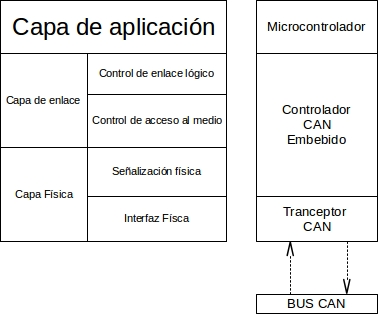
\includegraphics[scale=0.5]{images/Marco_teorico/ISO11898_Arquitectura_Standar.jpg}
  \caption{Arquitectura estándar propuesta por ISO898}
\label{fig:iso11898}
\end{figure}

En resumen, la capa física de CAN  describe la definición del bit timing, bit enconding y la sincronización, los niveles aceptables de la señal (corriente y voltaje), los conectores y características físicas de los cables \citep{texasCAN}. Por otro lado la capa de enlaces de datos, provee todos los servicios necesarios para la transmisión de un stream de bits desde un nodo a otro.

El bus CAN es un bus de tipo broadcast, es decir que todos los nodos escuchan todas las transmisiones. No hay manera de enviar un mensaje a un determinado nodo, por lo tanto no es necesario el direccionamiento de nodos. \citep{kvaserWEB}.

Actualmente la industria aeronáutica la utiliza. También el área agrícola en sus maquinarias, control de tráfico, sistemas de control industrial, sistemas domóticos y además, en equipamientos médicos.

\subsection{Elementos necesarios}
Como se puede observar en la Figura \ref{fig:iso11898}

Cada nodo conectado a la red necesita de
\begin{itemize}
\item \ac{CPU}, o microprocesador, que decida que mensajes debe recibir y que debe enviar
\item Controlador CAN, muchas veces integrado en el controlador, el cual recibe la serie de bits del bus. También es el encargado de transmitir mensajes (cuando se requiera), esto significa que al mensaje lo convierte en una serie de bits.
  \item Tranceiver, definido en el ISO 11898.
\end{itemize}


% \subsection{Capa física}
\subsection{Capa física}\label{subsec:capafisca}
El estándar de CAN define el bit enconding, el timing, y la sincronización. La capa física es la encargada de convertir 1 y 0 en pulsos eléctricos para enviar mensajes por el canal, y también el proceso inverso cuando recibe mensajes. La capa física es implementada enteramente en \ac{HW} \citep{texasFISICACAN}.

\subsubsection{Bus de comunicación}
Para iniciar una transmisión de mensaje es necesario como mínimo dos nodos conectados al bus CAN. Esto se debe a que el dispositivo que envía un mensaje está también recibiendo su propio mensajes, con esto puede chequear cada bit que ha enviado. De esta manera, un segundo nodo responde con un ACK, mientras el bit todavía está siendo transmitido por el primer nodo. Esto demuestra por qué se necesitan de dos nodos para completar la transmisión de mensajes \citep{texasFISICACAN}.

En la Figura \ref{fig:traficBUSCAN} se observa un ejemplo extraído de \citep{texasFISICACAN}. En esta se muestra un nodo A que envía un mensaje. Luego se ve que que B y C contestan con un ACK indicando que el mensaje fue recibido sin errores. Luego B y C comienzan a transmitir hasta que C gana el bus debido a que tiene un bit dominante, y termina este completando su mensaje.

\begin{figure}[h]
 \centering
 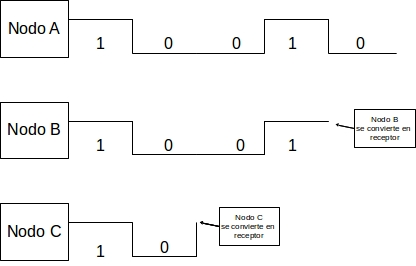
\includegraphics[scale=0.3]{images/Marco_teorico/CAN_BUS_Traffic.jpg}
  \caption{Tráfico en el BUS CAN}
\label{fig:traficBUSCAN}
\end{figure}

El medio físico  es una línea de bus con dos cable, terminada por una resistencia. Los cables pueden ser paralelos, trenzados y/o blindandos. Los segmentos de cable para la conexión de los nodos deben ser lo más cortos posibles.

Para mayores detalle técnico referentes al bus será necesario estudiar el estándar ISO 11898 o en \cite{texasFISICACAN}.

El largo del bus va a determinar el bitrate de la comunicación. Para alcanzar un bitrate de 1Mbps, el máximo del canal de comunicación es de 40m. Si se tiene un bus de 1km el bitrate es de 0.05Mbps. Con esto se puede observar que el bitrate decae cuando la distancia se incrementa. Para CAN, el bitrate también está determinado por el total del delay del sistema \citep{texasFISICACAN}. Esto es la suma de los delays del nodo, y el delay propio del cable.

Debe destacarse que que existen diferentes capas físicas para el protocolo CAN:
\begin{itemize}
\item El tipo más común es el establecido en el estanar ISO 11898-2. Este protocolo cuenta con dos cables, cada uno identificado como CAN\_H y CAN\_L. También es llamado \textit{CAN de alta velocidad} (1 Mbit/s). Este requiere que el largo del cable sea como máximo 40m.
\item También en el estándar de ISO se establece el ISO 11898-3, el cual define otro esquema de doble cable balanceado pero para bajas velocidades. Este es tolerante a fallas si alguno de los cables entra en corto circuito. También es llamado también como \textit{CAN de baja velocidad} (125 kbit/s)
\item Se define el SAE J2411 que utiliza un solo cable para la capa física. Este es utilizado en autos (velocidad por encima de los 50 kbit/s). No tiene demasiados requerimientos en cuanto al bitrate ni el largo del canal de comunicación. El estandar define 32 nodos por red.
\item Existen modificaciones del estandar RS485 para su funcionamiento con CAN
\end{itemize}

\subsubsection{Bit timing}
El tipo de señal es codificado con Non Return Zero (NRZ). Los bits son codificados en dos estados llamados ``recesivo'' y ``dominante''(el bit 0 es asociado al bit dominante). El protocolo pemite acceso al bus multi-master con una resolución determinística ante colisiones. Para lograr la sincronización, el protocolo sincroniza durante las transiciones. Por tal motivo, deben evitarse el envío de largas cadenas de bits en un mismo estado. CAN utiliza una técnica que se denomina ``bit stuffing'' o ``bit padding'' en la cual luego de enviar 5 bits con el mismo estado, se insertan bits de relleno.

\subsubsection{Asignación eficiente del bus}
La asignación del bus depende de su aplicación. Generalmente existen 2 tipos de clases de asignación.

\begin{itemize}
\item \textbf{Asignación en un tiempo fijo}: La asignación se hace secuencialmente a cada participante sin importar si este necesita el bus en ese momento. Esta técnica, asigna tiempo del bus a cada nodo, y si no tiene nada que enviar, el bus se encuentra ocioso.

\item \textbf{Asignación en base a sus necesidades}: el bus se asigna según las necesidades del nodo (utilizando CSMA o CSMA/CD). En CAN la asignación del bus es negociado entre los mensajes que esperan ser transmitido. CAN utiliza esta técnica.
\end{itemize}


% \subsection{Capa de enlace}
\subsection{Capa de Enlace}
CAN utiliza el control de acceso al medio tipo \textit{CSMA/CS+CR} (Acceso múltiple con detección de portadora, detección de colisión más resolución de colisión). CAN resuelve el problema de la colisión con la supervivencia de una de las tramas que chocan en el bus. La trama ``ganadora'' es aquella que tiene mayor prioridad. Por lo tanto se puede indicar que CAN por naturaleza tiene en cuenta la prioridad.

Como ya se mencionó anteriormente el bit \textit{dominante} es el 0 y el bit \textit{recesivo} es el 1, la resolución se realiza con una operación lógica AND de todos los bits transmitidos simultaneamente. Cada transmisor se encuentra continuamente
observando y comprobando que el bit recibido se corresponda con el bit que envía. Cuando no coincide, el controlador retira el mensaje del bus y se convierte automáticamente en receptor. Como puede observarse la capa de enlace se comparta de manera similar a la capa física.

La única diferencia que presenta la capa de enlace de CAN es que todos los errores a nivel de un solo bits son detectados. Los errores de múltiples bits son detectados con una alta probabilidad \citep{can-ciaWEB}.


% \subsection{Formato del mensaje}
\subsection{Formato del mensaje}
CAN utiliza un formato de mensajes cortos (94 bits) En el mensaje no está explícito ninguna dirección, por este motivo el mensaje puede ser escuchado por todos los nodos de la red \citep{kvaserWEB}.

Los tipos de mensajes son los siguientes:
\begin{itemize}
    \item Frame de datos (Data Frame)
    \item Frame remoto (Remote Framte)
    \item Frame de error (Error Frame)
    \item Frame de sobrecarga (Overload Frame)
\end{itemize}

\subsubsection{Data Frame}
Este es el frame más común. Las partes más importantes son:

\begin{itemize}
\item Campo de arbitraje, el cual determina la prioridad del mensaje
\item El campo de datos, que contiene desde cero hasta ocho bytes de datos
\item El CRC, que está conformado por 15 bits utilizados para calcualr el checksum del mensaje
\item Un campo de ACK. Cualquier controlador que haya recibido el mensaje envía un bit de acuse de recibo al final de cada mensaje. El transmisor comprueba la presencia del bit ACK. En caso de no detectar este bit reenvía el mensaje. Al no poder conocer la dirección de los nodos, no se sabe si el mensaje fue recibido correctamente por el node receptor, solo se sabe que el mensaje fue recibido por uno o más nodos.   
\end{itemize}

\subsubsection{Remote Frame}
El frame remoto es un Data Frame con dos diferencias, es marcado como Remote Frame, esto es el bit RTR es recesivo; y por otro lado no hay un campo de datos. Este frame es utilizado para pedir la transmisión de un determinado frame de datos. Por ejemplo si el nodo A transmite un Remote Frame con el campo de arbitraje en 234, entonces el nodo B, reponderá con un frame de datos con el campo de arbitraje seteado a 234 \citep{kvaserWEB}. Este frame es poco utilizado.

\subsubsection{Error Frame}
Este frame se envía cuando un node detecta alguna falla en el mensaje. El envío de este frame provoca la retransmisión inmediata del mensaje. El Error Frame consiste en una bandera, el cual está compuesto por 6 bits del mismo valor, y un Error Delimiter que está compuesto por 8 bits recesivos.

\subsubsection{Overload Frame}
Este frame es similar al frame de error con el mismo formato. Es enviado cuando el nodo está ocupado. Este Frame es muy poco usado. El único controlador que generaba Overload Frame está obsoleto \citep{kvaserWEB}


\subsubsection{CAN estándar y CAN extendido}



% subsection that talk about CANAerospace
\subsection{CANAerospace}\label{subsec:CANaerospace}
CANAerospace es una definición de protocolos y datos que fue diseñada
para ser utilizada en sistemas de comunicación altamente confiables,
sobre todo aeroespaciales, que estén basadas en el \ac{CAN}
\citep{CANAerospaceWEB}. Este, fue desarrollado por Stock Flight Systems,
creado en 1997 y tiene su primer Release en 1998, y fue utilizado en varias aeronaves,
como por ejemplo SOFIA Boeing 747SP\footnote{Ver: https://www.sofia.usra.edu/public/about-sofia/sofia-aircraft}.
También es utilizado en las interfaces de simuladores de vuelvo. 
CANAerospace es un proyecto open source, y se continúa desarrollando. Fue
publicado por NASA con el nombre de Advanced General Aviation Transport
Experiments Databus Standard (AGATE).

Este protocolo nace con el propósito de crear un estándar para la creación
de aplicaciones que requieran un constante monitoreo del flujo de datos y una
sincronización de tiempo en sistemas con redundancias \citep{CANAerospaceWEB}.


El protocolo CAN, por sí solo, no cubre problemas como la representación de datos,
direccionamiento, protocolo orientados a la conexión. Además, la utilización de CAN
en aplicaciones espaciales requieren de la definición de un estándar que esté
orientando a los requerimientos específicos de la misión. CANAerospace es creado
para enfrentar estos problemas. Este protocolo es una pequeña capa de software
que permite un manejo fácil del bus de datos que cumple con los requerimientos
específicos de sistemas de aviónicas. CANAerospace fue instalado en una gran cantidad
de aeronaves desde 1998 y ha demostrado  una excelente confiabilidad en
ambientes hostiles.

Algunas de las características más destacable de CANAerospace es que, no existen
esclavos y maestros, por ello se dice que es una red democrática. Los mensajes
se encuentran bien identificados. Existen mecanismos para informar eventos de
emergencias. Es sencillo de aplicar. Y  es un proyecto open source, por lo tanto
no tiene costo alguno, y existen tutoriales libres y gratuitos.

\subsubsection{Formato del mensaje CANAerospace}
En la Figura \ref{fig:CANAerospaceMessage} se puede observar el formato
básico del mensaje de CANAerospace. Este está compuesto principalmente
por cuatro  bytes, los cuales se describen a continuación:
\begin{itemize}
\item \textit{NODE-ID}: Este byte es utilizado cuando se produce un error en algún
  dispositivo y comienza a funcionar su redundancia. De esta manera, para aquellas
  arquitecturas que lo permiten, el protocolo puede identificar estos cambios.
\item \textit{Data-Type}: CANAerospace permite múltiples tipos de datos para cada mensaje.
  Este byte permite identificar cada tipo de datos de cada mensaje.
\item \textit{Service Code}: Para datos que se utilizan en las operaciones
  normales. Este dato debe reflejar el estado de los datos, esto ayuda a la
  implementación de un monitoreo integral de datos.
\item \texit{Message Code}: El número de mensajes permite detectar si el mensaje
  se perdió y verificar si la unidad de transmisión trabaja correctamente. 
\end{itemize}

\begin{figure}[h]
 \centering
 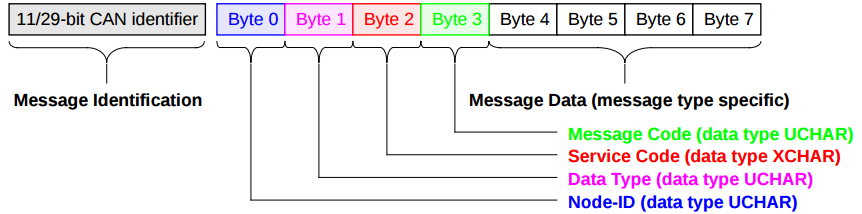
\includegraphics[scale=0.5]{images/Marco_teorico/CANAerospace_Message.png}
  \caption{Formato del mensaje de CANAerospace}
\label{fig:CANAerospaceMessage}
\end{figure}





\vspace{1cm}
\noindent\rule{\textwidth}{2pt}

\textbf{\Large{Resúmen}}

En este capítulo se desarrollaron diferentes conceptos que son importantes ya que sustentan
este trabajo de tesis.

Los principales conceptos que se necesitan conocer son:

\begin{itemize}
\item \textbf{Avería} de sistema ocurre cuando el servicio prestado por el sistema ya no coincide con las especificaciones del mismo. Esto quiere decir que existe un problema que tiene
una consecuencia negativa en el sistema completo, logrando que este ya no logre cumplir con sus
especificaciones
\item Un \textbf{error} es una parte del estado del sistema
que es susceptible de provocar un avería en el sistema. Un error que afecta al servicio, es una
indicación de que un avería se ha producido.
\item La causa adjudicada o la hipótesis de un error es una \textbf{falla}, también llamado ``bugs''. Una falla es un defecto que está presente en el sistema y que puede causar un error. Es la desviación actual de lo correcto \cite{Hanmer07}.
\end{itemize}

Por otro lado, la fiabilidad también se la puede considerar como una propiedad global que permite justificar la confianza de los servicios de un sistema. Esta puede ser clasificada en:
\begin{itemize}
\item Impedimentos, que son todas las cosas que se interponen en la fiabilidad de un sistema.
\item Medios, son los medios para lograr la confiabilidad. 
\end{itemize}

Los medios de la fiabilidad son los siguientes:
\begin{itemize}
\item Evitación de fallas, que son técnicas de mejoramiento de la fiabilidad utilizada durante el
desarrollo de software para reducir el número de fallas introducidas durante esta etapa.
\item Tolerancia de fallas, es la capacidad de un sistema a continuar funcionando a pesar de la ocurrencia de fallas.
\item Eliminación de fallas, son técnicas utilizadas para mejorar la fiabilidad, que se
emplean durante la validación y verificación del sistema.
\item Predicción de fallas, esto se lleva a cabo mediante una evaluación del comportamiento del
sistema con respecto a la ocurrencia o la activación de una falla. 
\end{itemize}

Los atributos de la fiabilidad son los siguientes:
\begin{itemize}
\item Confiabilidad, es la probabilidad de que un sistema continúe operando correctamente
durante un intervalo de tiempo dado.
\item Disponibilidad, la disponibilidad \textit{A(t)} de un sistema en el
instante de tiempo \textit{t} es la probabilidad que el sistema esté funcionando correctamente en
el instante \textit{t}.
\item Seguridad, es definida como la probabilidad que el sistema sea capaz de realizar sus funciones correctamente o discontinuar sus funciones en una manera a prueba de fallas.
\end{itemize}

En este trabajo de tesis se trabaja con el protocolo CAN. Este fue desarrollado por Bosh en 1983, para ser aplicado en la industria automotriz, como respuesta al rápido crecimiento de la electrónica en el fabricación de automóviles. Fue estandarizada por la Organización Internacional de Estandarización (ISO) bajo el nombre de  ISO 11898. Este protocolo se definió con el objetivo de proveer comunicación determinística de sistemas distribuidos, y que necesiten un alto grado de confiabilidad. CAN permite la conectividad vía bus serial.

Las características de CAN que la convierten en un tentadora opción para la aplicación en el sector espacial, son:
\begin{itemize}
  \item Bajo costo
  \item Operabilidad en ambientes eléctricos complicados
  \item Capacidades de tiempo real.
  \item Facilidad en el uso
\end{itemize}
